\documentclass[12pt]{article}
% Margin fixes
\oddsidemargin -0.5in
\evensidemargin -0.5in
\textwidth 7.25in
\topmargin 0.0in

\headheight 0.0pt
\headsep 0.0pt
\voffset 0.0pt
\textheight = 9.0in
\usepackage{amsmath,amssymb,graphicx,float}

\title{Millikan Oil Drop}
\author{Nathan Grouse\\Lisa Tran}

\newcommand{\counts}{\text{ counts}}

% Start the document!
\newcommand{\documentname}{\textsl{Article}}
\begin{document}
\maketitle

\section{Introduction}
\indent \indent To recreate Robert Millikan's Oil Drop experiment. This is done by monitoring the motion of a single oil droplet being acted on by vertical electrical forces in a closed chamber.

\subsection{Apparatus}
\indent \indent The apparatus includes a closed chamber for the oil droplets with a hole on top, a vial of oil with a nozzle and squeeze pump, a halogen lamp - this was switched a few times during the experiment because of bulb issues - for illuminating the chamber, and a viewing scope to magnify and track oil droplets on a grid inside the chamber. There are many other pieces to the apparatus, but these are most prominently used.

\section{Theory}
\indent \indent These are descriptions of the motion of an oil droplet in the chamber down and up respectively:
\[ mg = kv_f \]
\[ Ee_n = mg + kv_r \]
\indent \indent Then they skip a short derivation after eliminating k and solving for $e_n$:
\[k = \frac{mg}{v_f} \]
\[k = \frac{Ee_n - mg}{v_r} \]
\[mgv_r = (Ee_n - mg)v_f \]
\[e_n = \frac{mg(v_f + v_r)}{Ev_f} \]
\indent \indent The rest of the derivation of the expression for the charge of a droplet is straightforward geometry and substiution with the exception of an application of Stokes' Law, relating the radius of a sphere to it's velocity, and the addition of a correction factor to account for an assumption made in deriving Stokes' Law.
\[e_n = ([4 \pi d/3][(9n/2)^3/\sigma g]^1^/^2)([1+(b/pa)]^3^/^2)((v_f + v_r)v_f^1^/^2 / V_p) \]

\section{Data}

\begin{figure}[H]
\centering
\hspace{-0.0in}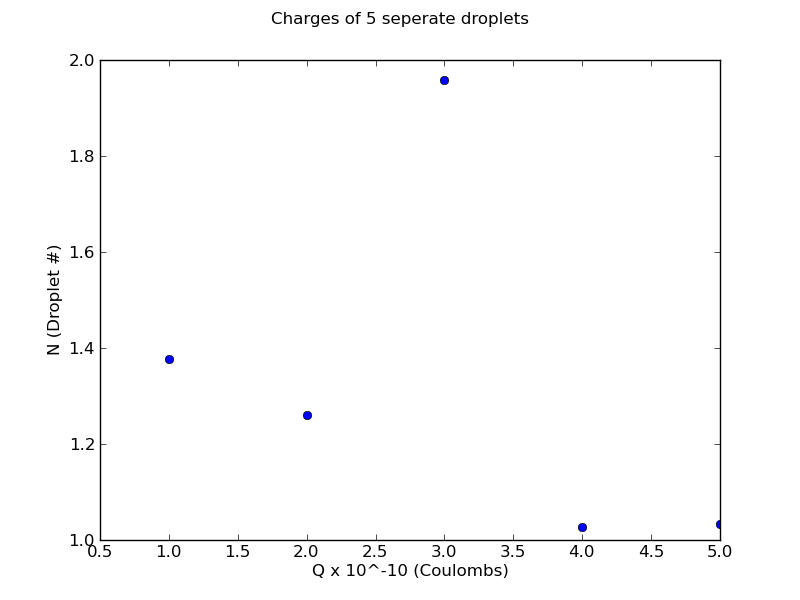
\includegraphics[scale=0.60]{Plot1.png}
\end{figure}

\begin{figure}[H]
\centering
\hspace{-0.0in}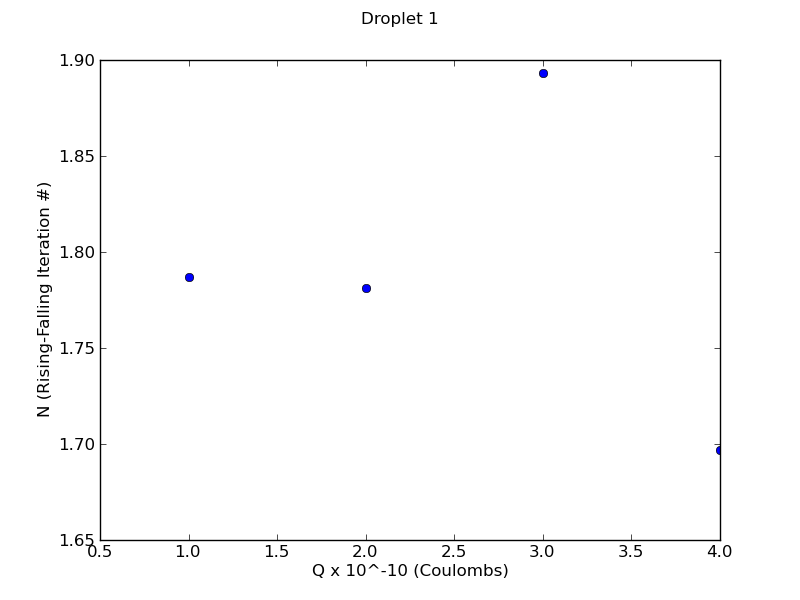
\includegraphics[scale=0.60]{Plot2.png}
\end{figure}

\begin{figure}[H]
\centering
\hspace{-0.0in}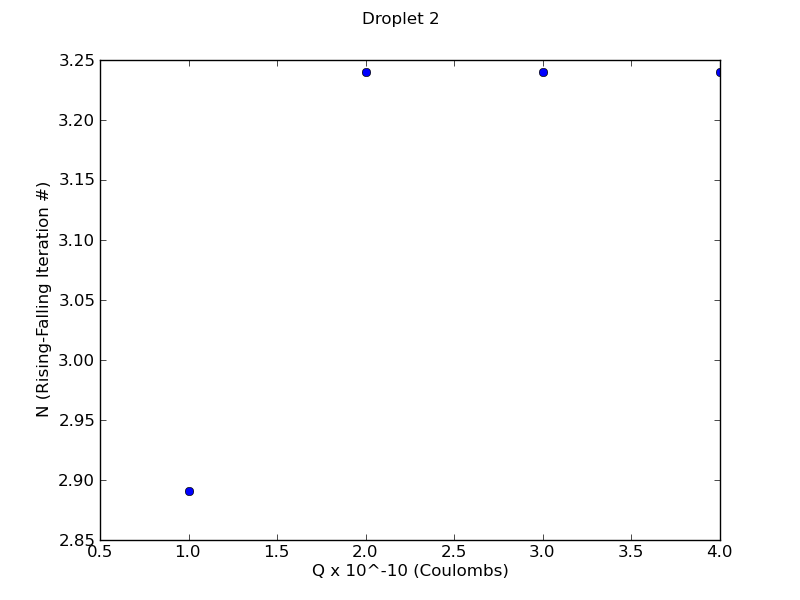
\includegraphics[scale=0.60]{Plot3.png}
\end{figure}

\section{Error Analysis}
\indent \indent These calculations for the charges of the droplets are not ordered or on the expected order of magnitude. Any given droplet should only have a small number of excess electrons, which would result in some net charge on the order of $10^-^1^9$. A percent error would only emphasize how far from expected these results are. The instructions for this lab mention that to successfully measure the charge of an electron, the experimenter must have some degree of skill for choosing an appropriate oil droplet and the ability to change the charge on that droplet. My partner and I were not even able to keep one oil drop in sight for four iterations of falling and rising. The error is most likely due to human error in data gathering, or my own computational error - though I have repeated these computations a few times in hopes of calcuating a more accurate result.

\section{Conclusion}
\indent \indent I did not obtain reasonable results. Though I didn't see what I expected to see in the data, the experiment itself seemed to be working just fine and there was no apparent equipment failure.

\end{document}